%\chapter{Il potente e saggio Fabio Fazio nel magico mondo di LHC}
%Forse, non tutti sanno che, Fabio Fazio, un po' come Britney Spears e i semiconduttori, \'e un grande appassionato di rivelatori di particelle al punto di possederne uno piccolino nei suoi appartamenti di Celle Ligure. Il Fazio \`e molto esperto e molto bravo a riconoscere tutti quei rivelatori ridondanti, pieni di boria e faziosi da quelli utili come quelli del CERN. Come Dante scelse Virgilio per accompagnarlo nel suo viaggio attraverso l'aldil\`a io mi affido a lui affich\`e possa essermi guida e consiglio nel fazioviaggio in quel di LHC e dell'esperimento ATLAS.

%Now the serious part begins. {\scshape Please, read from here.}
\chapter{The LHC and the ATLAS experiment}
\lettrine{T}{his} analysis uses data collected during 2015 and 2016, coming from the ATLAS detector at LHC, as well as all simulations were performed in its context. It is a good thing to begin this work describing the main features of the LHC facility at CERN and giving an overviwew of the ATLAS experiment. 

\section{The Large Hadron Collider}
Since the day of its starting up LHC (Large Hadron Collider) became the most powerful accelerator, of any kind, in the world. Built beneath the CERN site in Geneva, Switzerland, it consists of a double ring of \SI{27}{\km} lenght made of superconducting magnets in which hadrons (protons or heavy ions) can be accelerates nearly up to the speed of light, or $\gamma\simeq7500$, and forced to collide in 4 specific points where the two rings intersects and likewise detectors take place.

After the Higgs Boson discovery there are many open questions in physics that LHC is trying to give an answer. Up to now, the main target of this project are:
\begin{description}
\item[Supersymmetric discoveries] Despite the Standar Model of particle physics (SM) is a well established theory it doesn't provide a theory for gravitation similar to those for the other forces. A hint might come from supersymmetry (SUSY) that hypothesizes more massive particle than the ones we already know.
\item[Dark matter] Cosmological and astrophysical observations have shown that all visible matter accounts only for about 5\% of the mass/energy of the Universe. There are many experiment which tries to understand the nature of potential dark matter.
\item[SM particle property] A lot of properties of already known SM particle have to be defined with more precision. Since the production rate of \Wboson and \Zboson is high it is quite easy to verify any sort of deviation from SM predictions from this measurement and find prediction of new physics.
\item[Antimatter puzzle] LHC will also helps to investigate the matter/antimatter ratio. Even if after the Big Bang they have been produced in equal amount there is no explanation on why, as best of our knowledge, matter dominates the universe
\item[Quark-gluon plasma] Heavy ion collision at high energy, in which temperature can exceed the center of the Sun, can produce a state of plasma in which quarks are free. In this state detectors can study how the matter we know, in form of protons and neutrons in which confinement of quarks took place, has formed.
\end{description}

\subsection{\pp collision}
The most frequent collisions at LHC happen between protons. Before getting into the double ring they come across several machines which provide the first step of acceleration.

Protons are obtained from ionized hydrogen and accelerated by Linac2 up to \SI{50}{\MeV}, then injected into the Proton Synchrotron Booster (PSB), which accelerates them to \SI{1.4}{\GeV}. Then the beam travels into the Proton Synchrotron (PS), where is pushed towards \SI{25}{\GeV}, and into the Super Proton Synchrotron (SPS),  the second largest machine among all CERN's complexes consisting of a ring of \SI{1.1}{\km} radius, that speed the protons up to \SI{450}{\GeV}, which is the minimum at which the LHC can maintain a stable beam. The main advantage in using protons instead of electrons and positron, as it was used to in LEP at CERN before LHC, is thanks to their higher mass that they reduce syncrotron radiation while being accelerated. Protons are delivered in bunches: each bunch contains \SI{e11} of them and every proton beam has 2808 bunches. A simple representation of protons journey to LHC is given in \Fig{\ref{fig:accelerators}}.

\begin{figure}[tp]
	\centering
	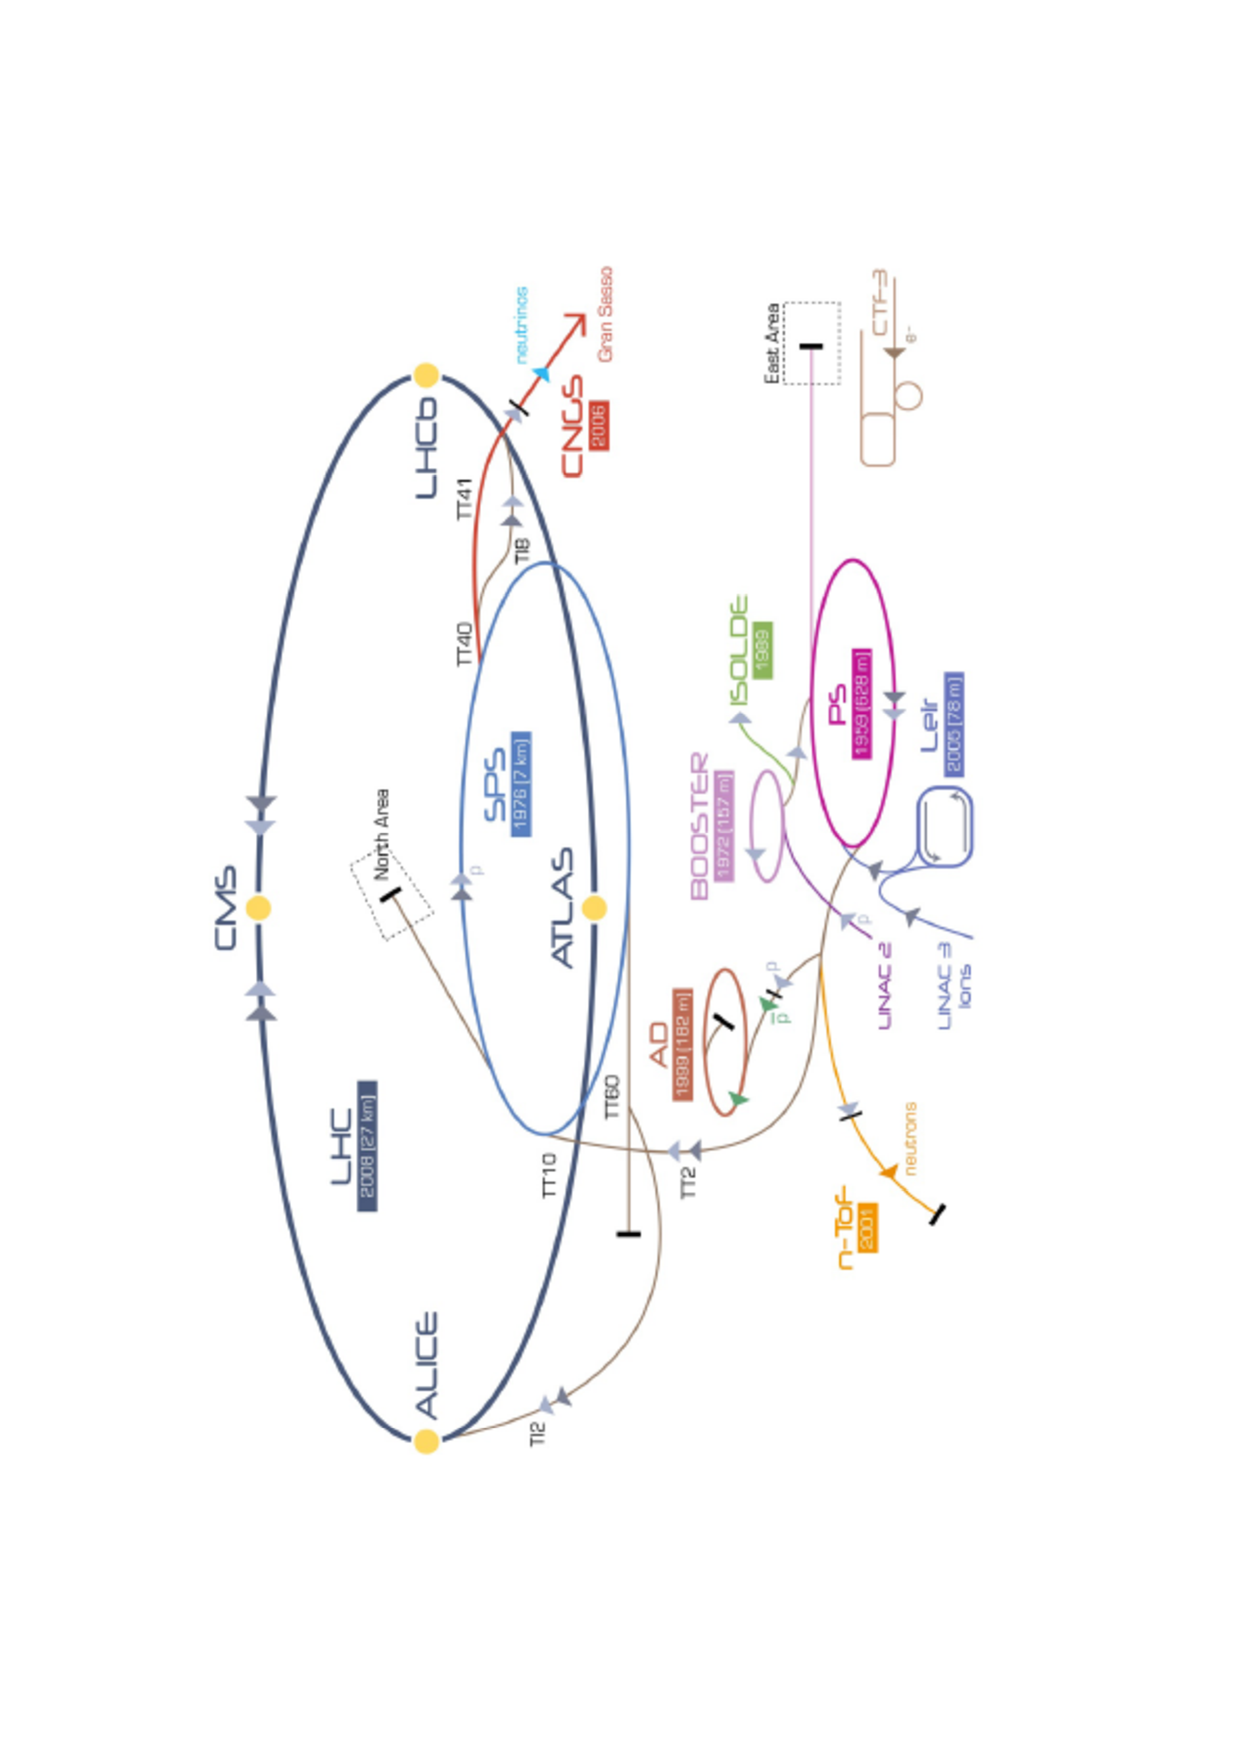
\includegraphics[width=0.75\textwidth,angle=-90]{LHC_ATLAS/CERNaccelerators}
	\caption{Simple sketch of the complex of the accelerators at CERN, from Linac2 to LHC}	
	\label{fig:accelerators}
\end{figure}

As mentioned earlier the LHC accelerator consists in a double ring complex of nearly \SI{27}{\km} lenght. It is made up of 8 arcs containing the dipole bending magnets and 8 insertion consisting of a long straight section plus two transition regions. The purpose of the magnets, made of superconducting material such as Niobium-titanium or Niobium-tin (\ce{Nb_3Sn}), is to provide to the beam a stable orbit: dipole magnets keep the particles in an almost circular orbit (even when it is bent by the Moon) and quadrupole magnets focus the beam. There is a third type of magnet used before making a collision to enhance its probability. Acceleration is provided by radiofrequency resonant cavities which also keep the beam at a constant energy compensating for energy losses and distribute the protons in bunches. so that every bunch is divided by \SI{25}{\ns} from another. LHC uses 8 cavities per beam each delivering \SI{5}{MV\per\m} at \SI{400}{\MHz} giving the beam \SI{500}{\keV} every turn. The cavities operate at \SI{4.5}{\K} while magnets are kept at \SI{1.9}{\K} by superfluid helium providing a magnetic field of \SI{8}{\tesla}.
In order to to avoid collision between hadrons and gas particles in the tubes, vacuum has to be made in them down to a pressure of \SI{e-13}{atm}.

\begin{table}[tp]
	\centering
	\begin{tabular}{lc}
	\toprule
	Quantity& Amount\\
	\midrule
	Circumference& \SI{26659}{\m}\\
	Dipole operating temperature& \SI{1.9}{\K}\\
	Energy, protons& \SI{6.5}{\TeV}\\
	Energy, heavy ions& \SI{2.56}{\TeV\per \amu}\\
	Peak magnetic dipole field& \SI{7.74}{\tesla}\\
	Distance between bunches& $\sim$ \SI{7.5}{\m}\\
	Peak Luminosity (protons)&  \SI{2.06e34}{\per \cm \squared \per \s}\\
	Designed Luminosity (heavy ions)& \SI{e27}{\per \cm \squared \per \s}\\
	No. of bunches per proton beam& 2808\\
	No. of protons per bunch (at start)& \SI{1.2e11}{}\\
	Number of turns per second& \num{11245}\\
	Number of collision per second& $\sim$\SI{4e7}{}\\
	\bottomrule
	\end{tabular}
	\caption{Table listing the main features of LHC}
\end{table}

The LHC was designed to operate with a \cm energy of $\sqrt{s}=\SI{14}{\TeV} $ for protons, even if this energy has not been reached yet, and \SI{1150}{\TeV} (or \SI{5.12}{\TeV\per\amu}) for heavy ions, and a rate of collision of \SI{e34}{per \cm \squared \per \s}, express in term of instantaneous luminosity. 
\clearpage
At LHC the insantaneous luminosity is computed via the formula:
\begin{equation}
	\mathcal{L}=\frac{f_{\textup{LHC}} \cdot n_{\textup{b}} \cdot N_{\textup{bunch}}^2}{A}
\end{equation}

where $f_{\textup{LHC}}$ is the collision frequency, $n_{\textup{b}}$ is the number of bunch colliding, $N_{\textup{bunch}}$ is the number of particle per bunch, where we are considering the approximate case in which both bunches share the same population. At last the inverse cross section of bunches is $A=4\pi\sigma_x\sigma_y$ where $\sigma_k$ are the r.m.s of the distribution of the beams along the transverse plane. Instantaneous luminosity can be increased for example by reducing the bunch section or increasing the number of protons per bunch even if it's not very wise for the rising of effects discussed soon.

With the instantaneous luminosity one can forsee the number of event expected after a collision. Since the event rate is given by 
\begin{equation}
\Gamma\equiv\frac{dN}{dt}=\mathcal{L}\times\sigma,
\end{equation}
where $\sigma$ is the total \pp cross section which at $\sqrt{s}=\SI{13}{\TeV}$ is about \SI{80}{mb}, we expect a rate of about \SI{e9}{\per\s}, or \SI{1}{\GHz}. Along with istantaneous luminosity an integrated luminosity is defined by simply integrating on time both members of the previous equation, in formul\ae:
\begin{gather}
	L=\int{\mathcal{L}dt} \notag\\
	N=L\times\sigma
\end{gather} 

\begin{figure}[tp]
	\centering
	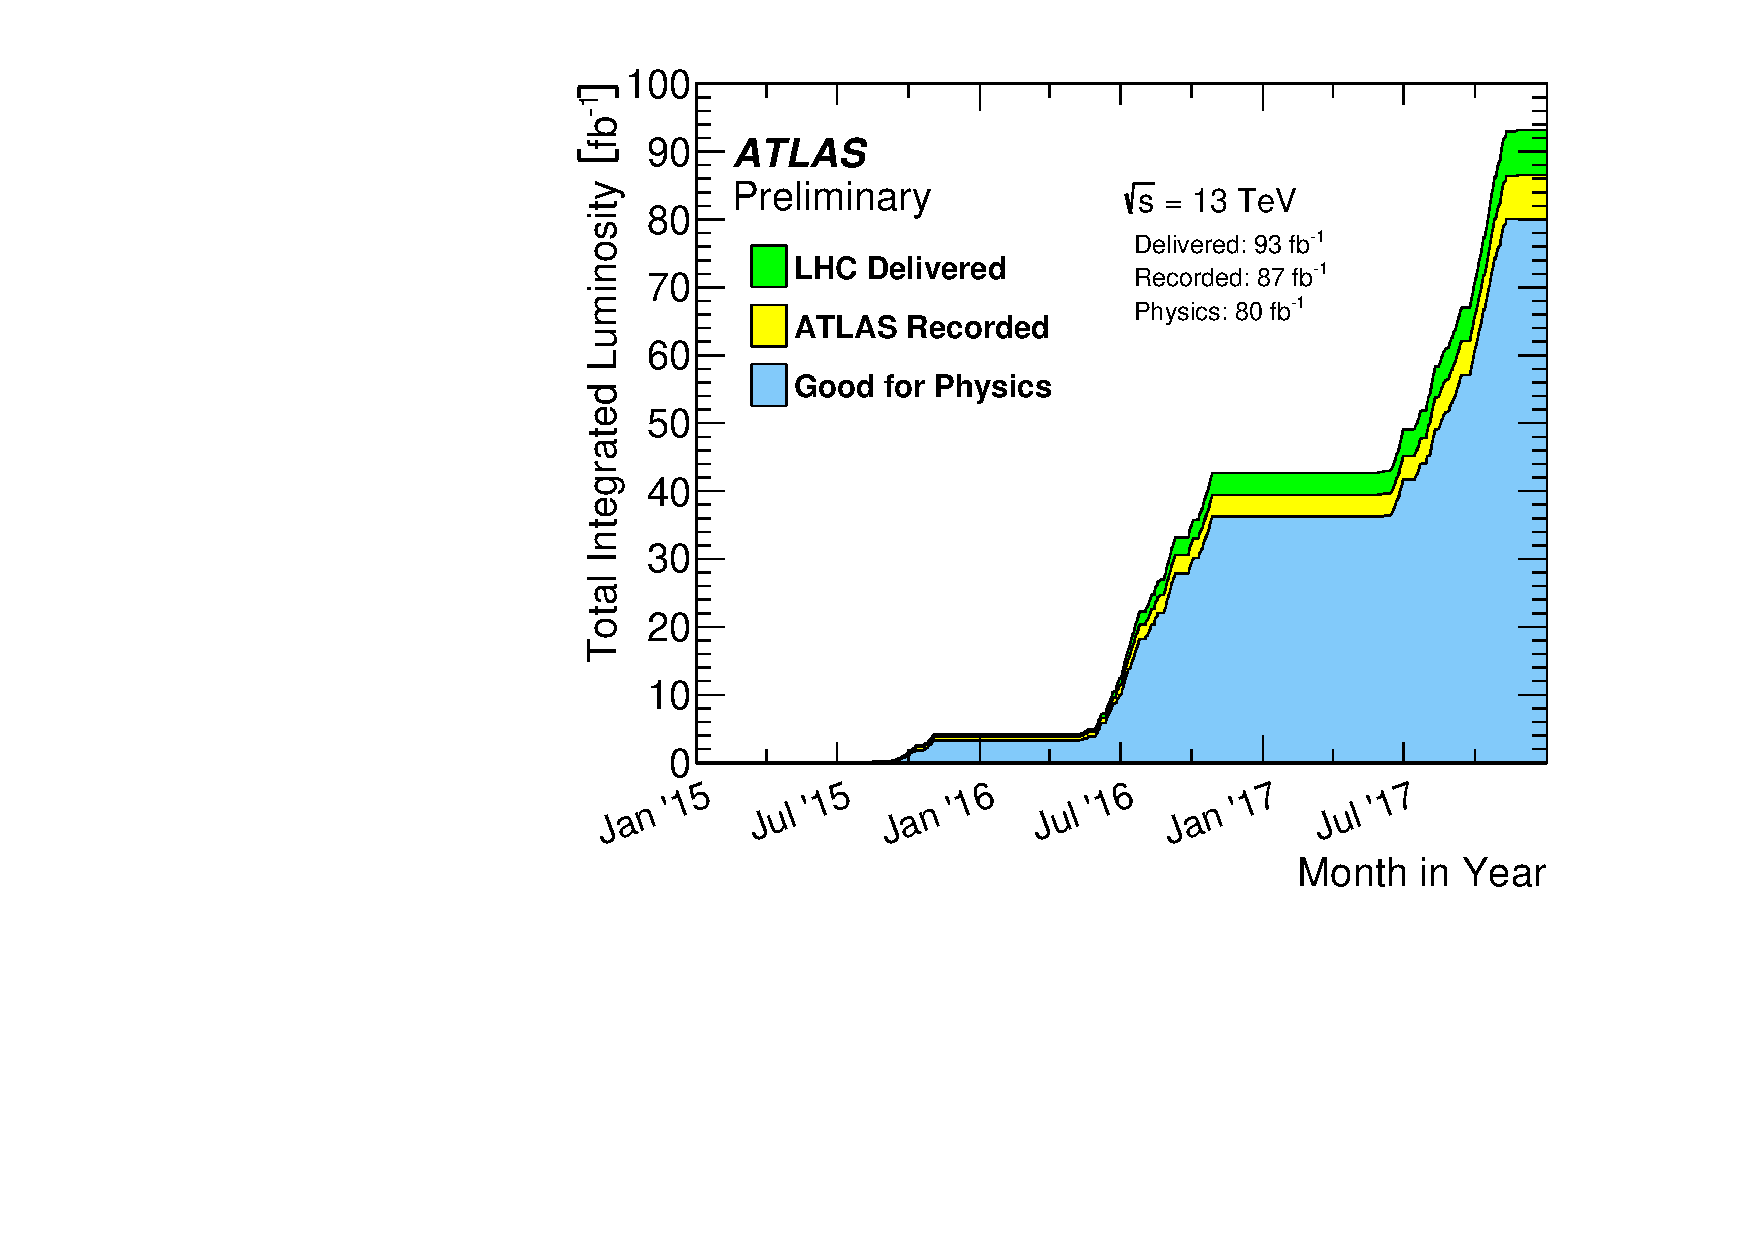
\includegraphics[width=0.75\textwidth]{LHC_ATLAS/intlumivstimeRun2DQ.pdf}
	\caption{Cumulative luminosity versus time delivered to ATLAS (green), recorded by ATLAS (yellow), and certified to be good quality data (blue) during stable beams for pp collisions at \SI{13}{TeV} \cm energy in 2015-2017.}
\end{figure}

Among this events one can distinguish \emph{soft collisions} and \emph{hard collisions}.
\begin{description}
\item[Soft collisions] These are the most frequent collision happening between two protons behaving like elementary particle. The momentum transfered is relatively small so that products of the collision scatter for a little polar angle. They have large longitudinal \mbox{momentum}, but small transverse momentum \pt of about \SI{500}{\MeV}.
\item[Hard collisions] Even though they are very rare, they occur at most once for every bunch crossing, they are the most relevant collision to be taken into account: products of most analysis interest come from them. In this kind of collision the interaction happens at the quark size. The energy involved is made up also from parton momentum which is not known \emph{a priori}, but can be extimated from the Parton Distribution Function (PDF) giving the distributions of quark and gluon momenta inside the proton. From hard scattering we can get particle with high \pt with eventually high mass.
\end{description}

What a detector see is always a superimposition of this two kind of scattering. The principal source of noise in the detector comes from \pileup interactions, i.e. additional \pp collisions that are recorded as belonging to the same event, but are in fact originated by distinct collisions. It can be distinguished in \emph{in time \pileup} when multiple interaction comes from the same bunch crossing and \emph{out of time \pileup} when previous scattering left any electronic signal in the detector which overlap with the one from successive collisions. In order to avoid this unpleasant situation, LHC detectors have been built along a \emph{fast response time} cryterium so they do not integrate signal over many bunch crossing per time

\textbf{Manca underlying event}

\section{The ATLAS detector}
\begin{figure}[tp]
	\centering
	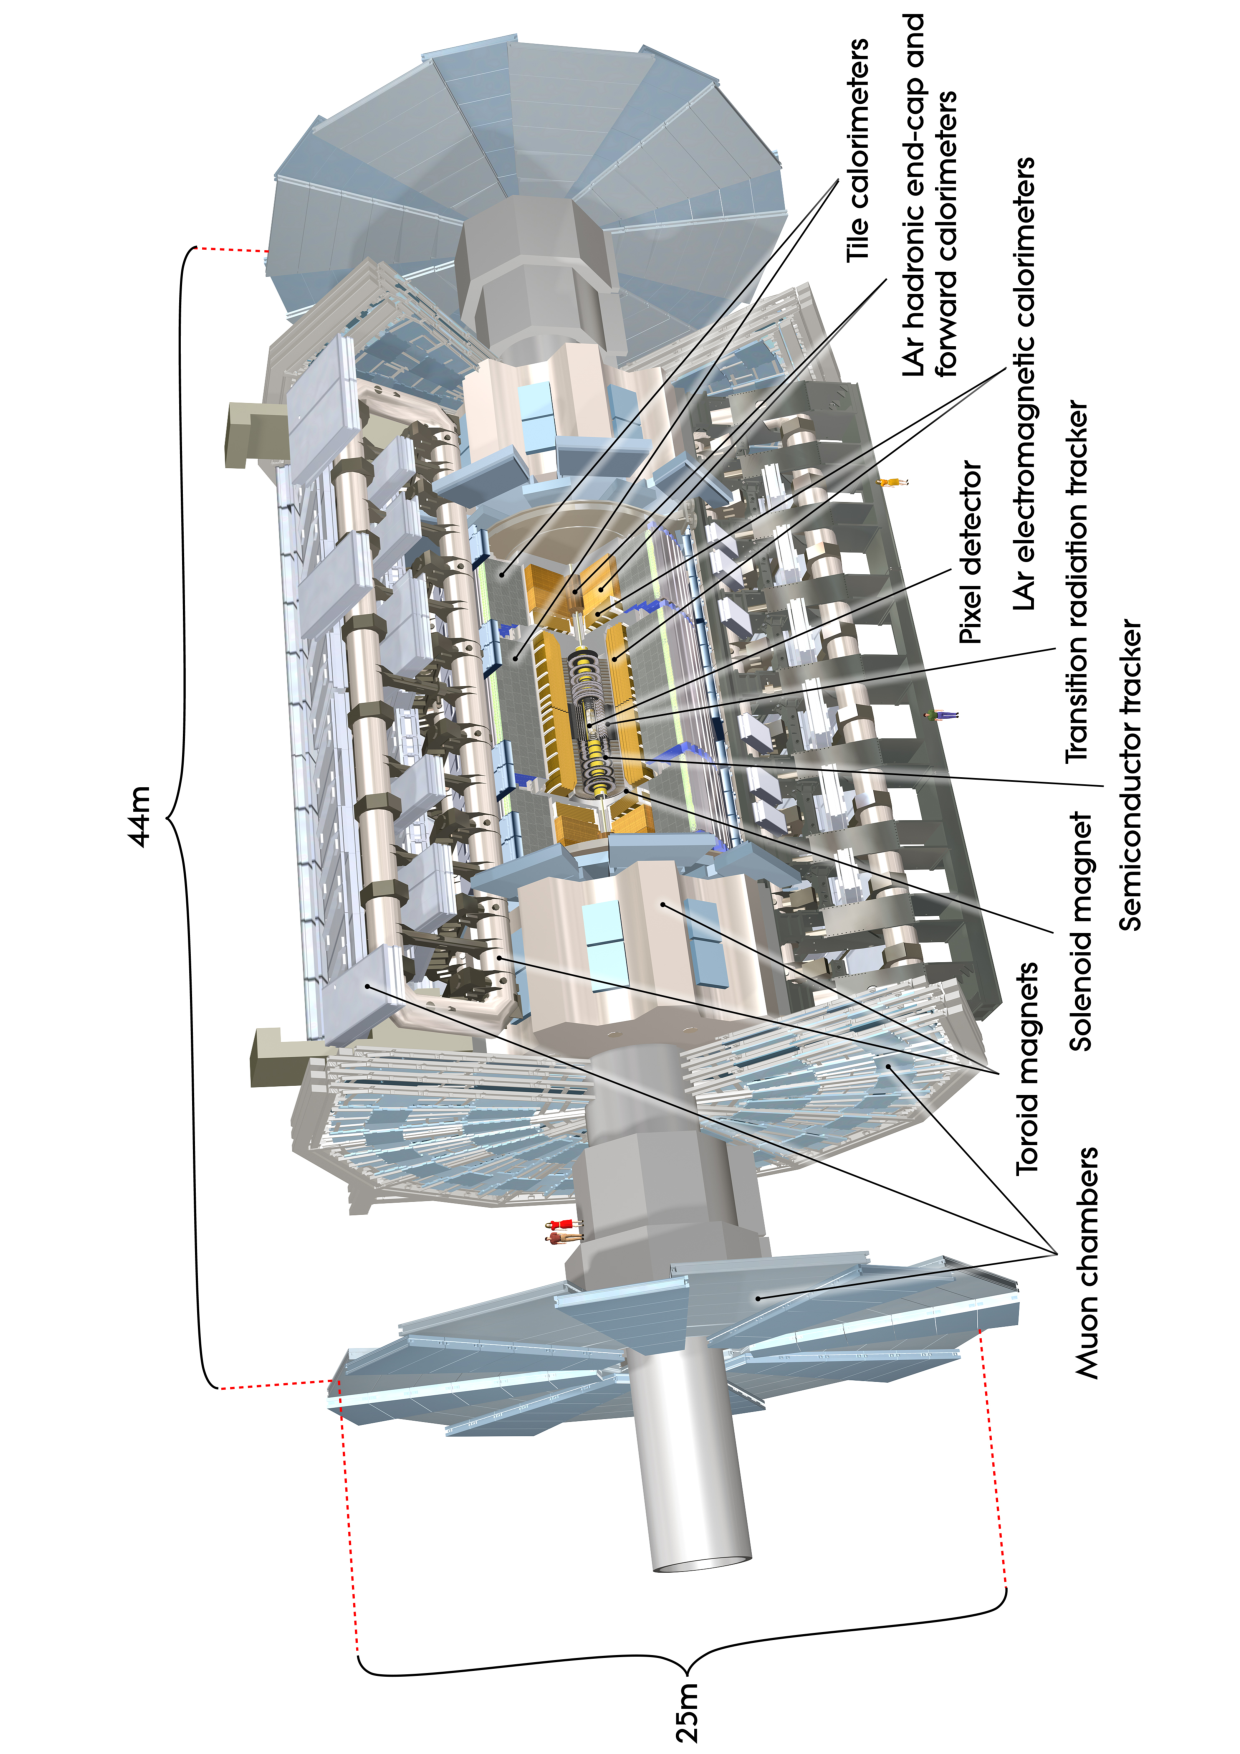
\includegraphics[scale=0.4,angle=-90]{LHC_ATLAS/0803012_01}
	\caption{Cut-away view of the ATLAS detector. The dimensions of the detector are 25 m in height and 44 m in length. The overall weight of the detector is approximately 7000 tonnes.}	
	\label{fig:atlas}
\end{figure}
ATLAS is A Toroidal Large ApparatuS being part of the four most important detector build around the LHC which are ATLAS, CMS, ALICE and LHCb. ALICE is a detector specialized in measuring and analysing lead-ion collisions, LHCb studies the asymmetry between matter and antimatter in $B-$particle while CMS and ATLAS are two \emph{general-purpose} experiment aiming to similar goals but with different technical solutions. A detailed description of the ATLAS experiment is given in \cite{atcollab:jinst}.

\subsection{Coordinate system}
The frame of reference used in ATLAS is very simple and it considers its origin in the nominal point of interaction. The \emph{z-}axis is defined along the beam direction so that the \emph{x-y} plane is orthogonal to it. The \emph{z} coordinate allows us to define two side of the detector: the \emph{A-side} where \emph{z} is positive and the \emph{C-side} where it's not. In the transverse plane the \emph{y-}axis points upwards and the \emph{x-}axis points towards the center of the LHC ring completing the right-handed triad. In the \emph{x-y} plane, which is the transverse plane, transverse momentum \pt and missing transverse energy \met, along with proper trasverse energy \et are defined.

Along with carthesian, one can also use polar coordinates to locate objects. The \emph{azimuthal} angle $\phi$ is measured around the beam axis starting from positive \emph{x} and proceeding counterclockwise, while the \emph{polar} angle $\theta$ is defined to be the angle from the beam axis. A simple sketch of the coordinate system used in ATLAS is described in \Fig{\ref{fig:coordinate}}.

It is often prefered to work with Lorentz-invariant quantities since collisions happen between partons whose boost is unknown. The rapidity $y$ transforms under Lorentz boost via a simple constant addition so that its difference is an invariant quantity. This quantity is used for massive objects like jets, when dealing with ultra-relativistic particle $y$ simplifies into the pseudorapidity $\eta$ which is trivially expressed in terms of the polar angle. In formul\ae:
\begin{gather}
	y=\frac{1}{2}\log{\frac{E+p^z}{E-p^z}}\\
	\eta=-\log{\tan{\frac{\theta}{2}}}
\end{gather}

Working with the pseudorapidity the $\eta	-\phi$ plane is defined. Distance in this plane are defined as:
\begin{equation}
	\Delta R=\sqrt{\left(\Delta \eta \right)^2 + \left(\Delta \phi \right)^2}
\end{equation}

Cones of constant pseudorapidity for notable value in ATLAS are highlighted in \Fig{\ref{fig:pseudorapidita}}. For last pseudorapidity helps to distinguish various region of the detector: the barrel (central) region which extends for \AetaRange{1.5}, the  end-cap region for \etaRange{1.5}{3.2} and the forward region which covers \etaRange{3.2}{4.9}

\begin{figure}[tp]
\footnotesize
\centering
	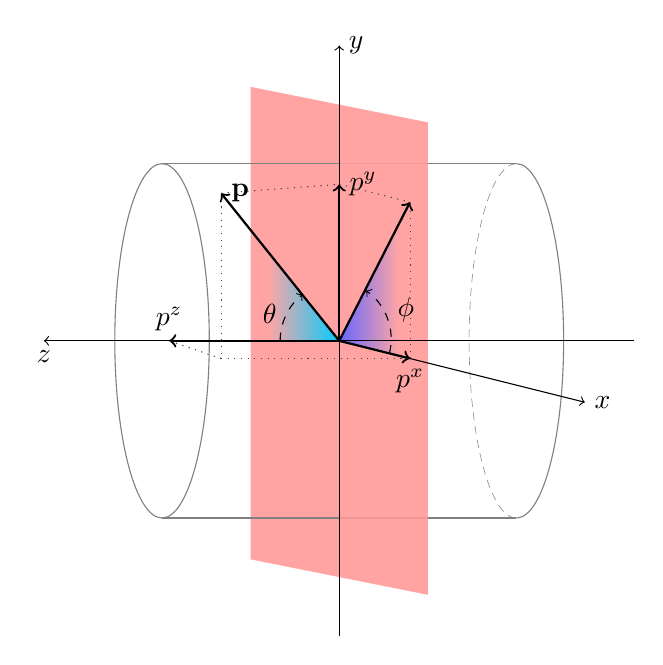
\begin{tikzpicture}[scale=0.75]
	
		\draw[gray] (-2.2,0) arc[x radius = 0.8, y radius = 3, start angle= 0, end angle= 360];
		\draw[gray] (3,3) -- (0,3); \draw[gray] (3,-3) -- (0,-3);
		\draw[gray,very thin,densely dashed] (3,3) arc[x radius = 0.8, y radius = 3, start angle= 90, end angle= 270];
		
		\draw[draw=none,fill=red!40!white,opacity=.9] (-1.5,4.3)--(1.5,3.7)--(1.5,-4.3)--(-1.5,-3.7)--cycle;

		\draw[gray] (3,-3) arc[x radius = 0.8, y radius = 3, start angle= -90, end angle= 90];
  	 	
  	 	\draw[gray] (0,3) -- (-3,3); \draw[gray] (0,-3) -- (-3,-3);
  	 	
  	 	
  	 	\draw[draw=none,  left color= blue!60!white, right color=red!35!white] (0,0)--(1,-0.25) -- (1,1.95) --cycle;
  	 	\draw[draw=none, right color= cyan!80!blue, left color=red!35!white] (0,0)--(-1.2,0) -- ( -1.2,1.53) --cycle;
  	 	\draw[->,dashed] (-1,0) arc [radius=1, start angle=180, end angle= 128] node[left =12pt, below]{$\theta$};
  	 	\draw[->,dashed] (0.85,-0.2125) arc [radius=1, start angle=-14.04, end angle= 55.3] node[below=7pt, right=8pt]{$\phi$};
  	 	
  	 	\draw[->,thick] (0,0)--(-2,2.5) node [right] {$\textbf{p}$};
  	 	\draw[->,thick] (0,0)--(1.2,2.35) node [right] {\textbf{\pt}};
  	 	\draw[->,thick] (0,0)--(-2.88,0) node [above ] {$p^{z}$};
  	 	\draw[->,thick] (0,0)--(1.2,-0.3) node [below ] {$p^{x}$};
  	 	\draw[->,thick] (0,0)--(0,2.65) node [right ] {$p^{y}$};
  	 	
  	 	\draw[thin,dotted,darkgray] (-2,2.5)--(-2,-0.3);
		\draw[thin,dotted,darkgray] (-2,-0.3)--(1.2,-0.3);
		\draw[thin,dotted,darkgray] (1.2,-0.3)--(1.2,2.35);
		\draw[thin,dotted,darkgray] (-2,2.5)--(0,2.65);
		\draw[thin,dotted,darkgray] (0,2.65)--(1.2,2.35);
		\draw[thin,dotted,darkgray] (-2,-0.3)--(-2.88,0);
		

		%===ASSI===
		\draw [->,thin] (5,0)--(-5,0) node[below]{$z$};
		\draw [->,thin] (0,0)--(4.16,-1.04) node[right]{$x$};
		\draw [->,thin] (0,-5)--(0,5) node[right]{$y$};
	
	\end{tikzpicture}
	\caption{Sketch of the frame of reference used in the ATLAS detector which is represented as a simple cilinder. The $z$ axis points along the beam, the $y$ axis points upwars and the $x$ axis points toward the center of LHC ring. The polar angle $\theta$ and the azimuthal angle $\phi$ are represented. The vector $\textbf{p}$ is decomposed in its component $(p^x,p^y,p^z)$ and its transverse part $\textbf{\pt}=p^x \textbf{e}_x+p^y \textbf{e}_y$ lying in the red transverse plane in the middle is pointed out.}
\label{fig:coordinate}
\end{figure}
\begin{figure}
  \centering 
  
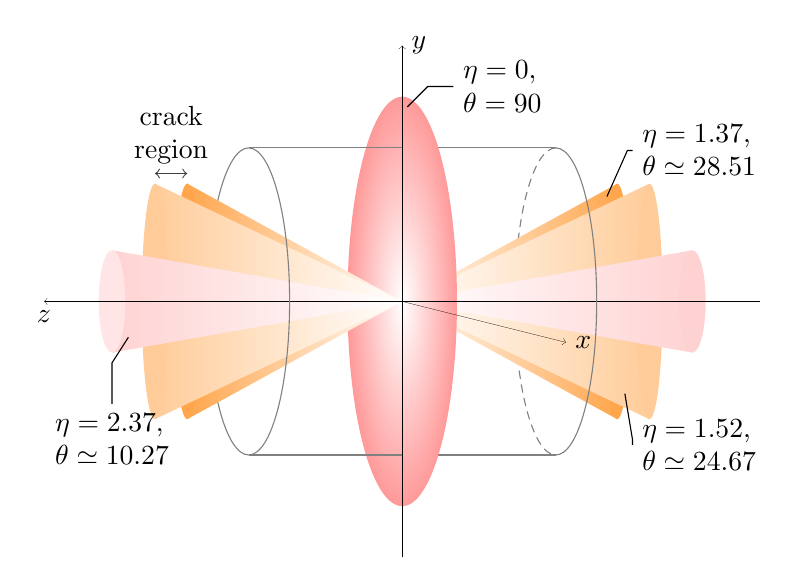
\begin{tikzpicture}[scale=0.65]
	\draw[gray,densely dashed] (3,3) arc[x radius = 0.8, y radius = 3, start angle= 90, end angle= 270];
	\draw[gray] (-3,3) arc[x radius = 0.8, y radius = 3, start angle= 90, end angle= 270];
	\draw[gray] (3,3) -- (0,3); \draw[gray] (3,-3) -- (0,-3);
	
	%eta1.37
	\draw[right color=orange!70!white, left color=white,draw=none] (0,0)--(4.2,2.3)--(4.2,-2.3) --cycle;
	\draw[fill=orange!70!white,draw=none] (4.2,2.3)arc[x radius = 0.26, y radius = 2.3, start angle= 90, end angle= 450];
	\draw[thin] (4,2.05) -- (4.4,2.95) -- (4.5,2.95) node[right,align=left] {$\eta=1.37$, \\$ \theta\simeq\ang{28.51}$};

	%eta1.52
	\draw[right color=orange!40!white, left color=white,draw=none] (0,0)--(4.83,2.3)--(4.83,-2.3) --cycle;
	\draw[fill=orange!40!white,draw=none] (4.83,2.3)arc[x radius = 0.26, y radius = 2.3, start angle= 90, end angle= 450];
	\draw[thin] (4.35,-1.8) -- (4.5,-2.7) -- (4.5,-2.8) node[right,align=left] {$\eta=1.52$, \\$ \theta\simeq\ang{24.67}$};
	
	%eta2.37
	\draw[right color=pink!70!white, left color=white,draw=none] (0,0)--(5.67,1)--(5.67,-1) --cycle;
	\draw[fill=pink!70!white,draw=none] (5.67,1)arc[x radius = 0.26, y radius = 1, start angle= 90, end angle= 450];

	
	%eta0
	\draw[inner color =white, outer color=red!40!white,draw=none] (0,0) ellipse (1.07 and 4);	
	\draw[thin] (0.1,3.8) -- (0.5,4.2) -- (1,4.2) node[right,align=left] {$\eta=0,$ \\$ \theta=\ang{90}$};
	
	%eta1.37left
	\draw[left color=orange!70!white, right color=white,draw=none] (0,0)--(-4.2,2.3)--(-4.2,-2.3) --cycle;
	\draw[fill=orange!70!white,draw=none] (-4.2,2.3)arc[x radius = 0.26, y radius = 2.3, start angle= 90, end angle= 450];
	
	%eta1.52left
	\draw[left color=orange!40!white, right color=white,draw=none] (0,0)--(-4.83,2.3)--(-4.83,-2.3) --cycle;
	\draw[fill=orange!40!white,draw=none] (-4.83,2.3)arc[x radius = 0.26, y radius = 2.3, start angle= 90, end angle= 450];
	
	%eta2.37left
	\draw[left color=pink!70!white, right color=white,draw=none] (0,0)--(-5.67,1)--(-5.67,-1) --cycle;
	\draw[fill=pink!40!white,draw=none] (-5.67,1)arc[x radius = 0.26, y radius = 1, start angle= 90, end angle= 450];
	\draw[thin] (-5.35,-0.7)--(-5.67,-1.2) -- (-5.67,-2) node[below,align=left] {$\eta=2.37$, \\$ \theta\simeq\ang{10.27}$};
	
	\draw[<->,darkgray] (-4.83,2.5)--(-4.2,2.5);
	\draw[] node at (-4.515,2.5) [above,align=center]{crack\\ region};
	%\draw[] node at (7.3,-0.3) [right,align=right]{$\eta=\infty,$\\ $\theta=\ang{0}$};

  	\draw [->,ultra thin] (7,0)--(-7,0) node[below]{$z$};
	\draw [->,ultra thin] (0,0)--(3.2,-0.8) node[right]{$x$};
	\draw [->,ultra thin] (0,-5)--(0,5) node[right]{$y$};
	\draw[gray] (-3,3) arc[x radius = 0.8, y radius = 3, start angle= 90, end angle= -90];
	\draw[gray] (0,3) -- (-3,3); \draw[gray] (0,-3) -- (-3,-3);
	
	\draw[gray] (3,-3) arc[x radius = 0.8, y radius = 3, start angle= -90, end angle= 90];

\end{tikzpicture}
\caption{Notable value of $\eta$ for the corresponding $\theta$. The crack region  for\etaRange{1.37}{1.52}, along with the limit of photon acceptance in this analysis for $\eta = 2.37$  are highlighted. The gray cilinder is a sketch of the ATLAS detector. Due to left-right simmetry, the $\theta$ angle displayed represent both the value shown and their $\pi-\theta$ symmetric. When $\theta$ approaches \SI{0}{°}, $\eta$ assumes larger values. }
\label{fig:pseudorapidita}
 \end{figure}

\subsection{General overview}
ATLAS geometry is mostly driven by its magnets: there is a thin superconducting solenoid surrounding the inner detector (ID), and provides a magnetic fields of about \SI{2}{\tesla}, and three superconducting toroids (one barre and two end cap) for every cilyndrical octant around the calorimeters. So ATLAS shows a forward/backward symmetry wrt the interaction point and an eightfold cilyndrical symmetry around the beam axis.

The ATLAS detector can be divided into three detectors, each one providing a precise task and accomplish a certain measurement for a specific class of particles.
\begin{description}
\item[Inner detector] Immersed in a solenoid, it provides to the pattern recognition, momentum and vertex measurements, and electron identification thanks to high-resolution semiconductor pixel, including the Insertable B-layer which was added before the start of \RunTwo, strip detectors in its inner part and straw-tube tracking detectors with the capability to generate and detect transition radiation in its outer part. It will be described in detail in \Sect{\ref{sec:ID}}.
\item[Calorimetry system] It is composed by two kind of calorimeter: a Liquid Argon (LAr) electromagnetic calorimeter and am hadronic calorimeter. They are surrounded by \num{24} toroidal magnet as described above and they provides to measure energy and track particle as their names suggest. It exhibit great position and energy resolution and it covers a very wide range in pseudorapidity extended by its forward part. For greater detail see \Sect{\ref{sec:calo}}.
\item[Muon spectrometer] The muon spectrometer surrounds the calorimeter. It provides muon momentum resolution which is achieved with three layers of high precision tracking chambers. It includes an air-core toroid system with a long barrel and two side end-caps, which bends muon trajectory. It is described in \Sect{\ref{sec:muons}}.

\end{description}

\subsection{Inner detector}
\label{sec:ID}
\begin{figure}[tp]
\centering
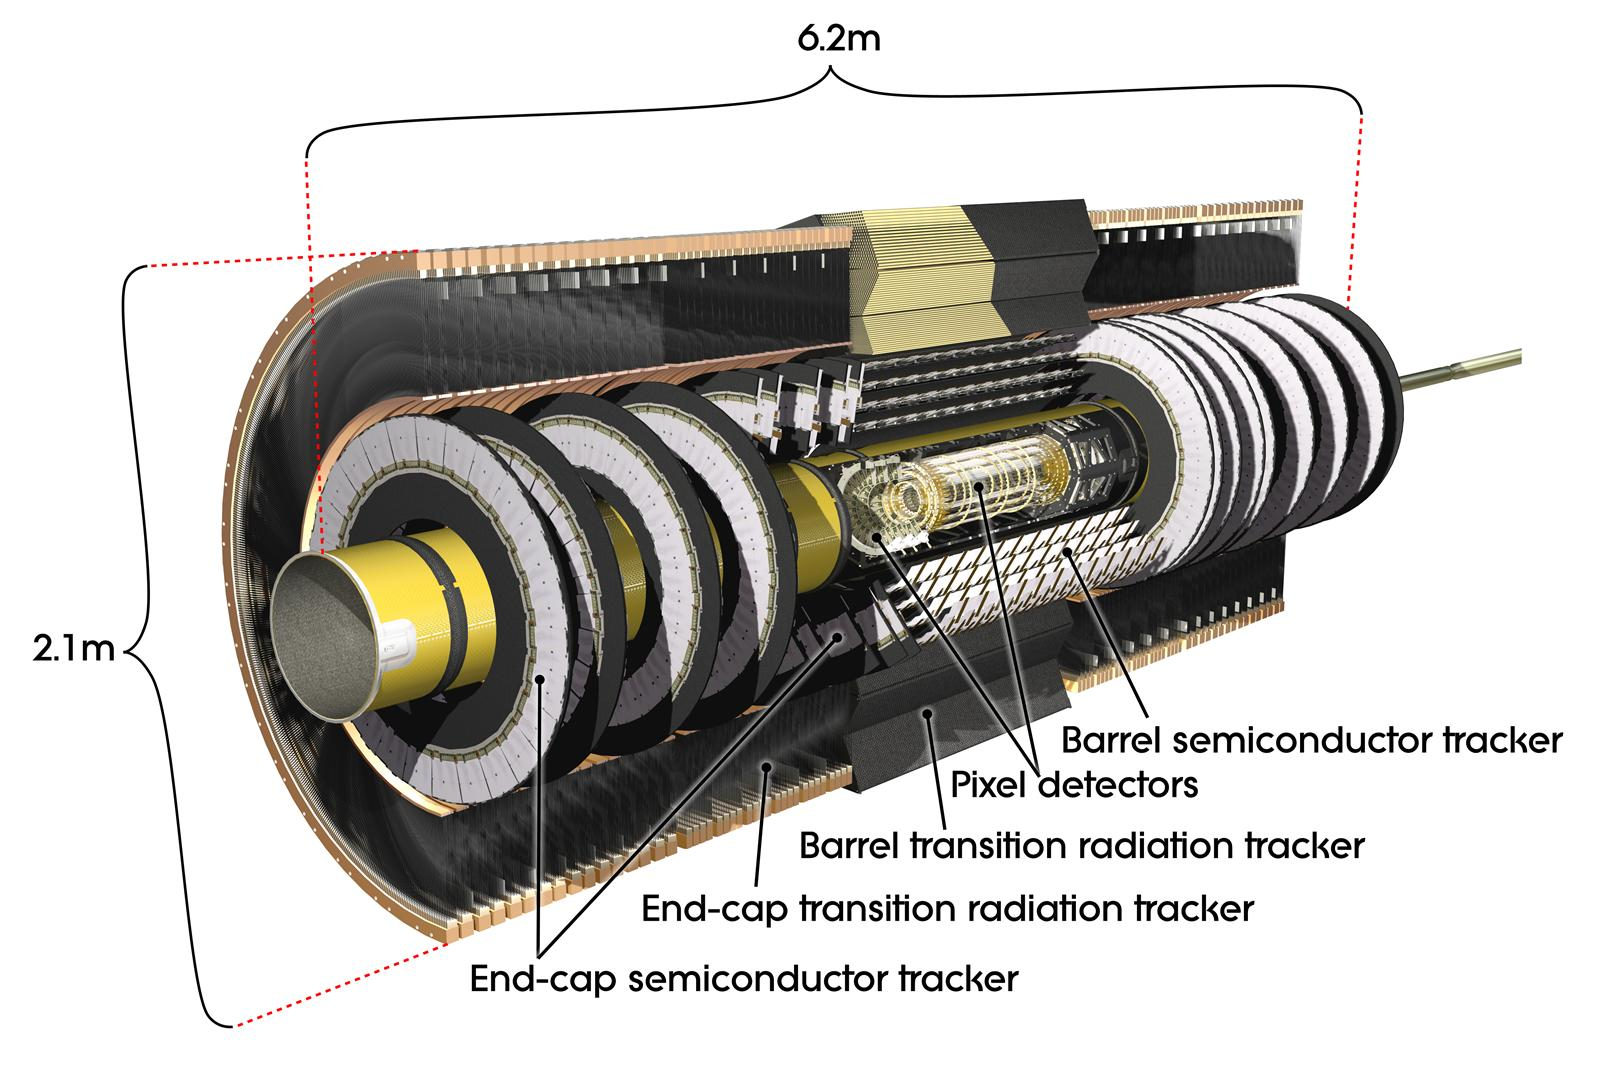
\includegraphics[width=0.8\textwidth]{LHC_ATLAS/ID}
\caption{Cut-away view of the ATLAS inner detector.}
\end{figure}

The inner detector (ID) is a tracking detector and it is designed to provide precise tracks recognition, excellent momentum resolution and both primary and secondary vertex measurements. For the purpose of tracking, great precision measurement must be performed so that an high granularity is strongly required. Indeed every \SI{25}{\ns} about \num{1000} particle emerge from a collision within a $\eta$ cone of \num{2.5}. Tracking charged particle is very crucial to help further detectors to distinguish between two similar particles. Showers left in the hadronic calorimeter by protons and neutrons are very similar, the only way we have to decide which particle has been detected is looking whether tracks were left in this region.

\begin{figure}[pt]
\centering
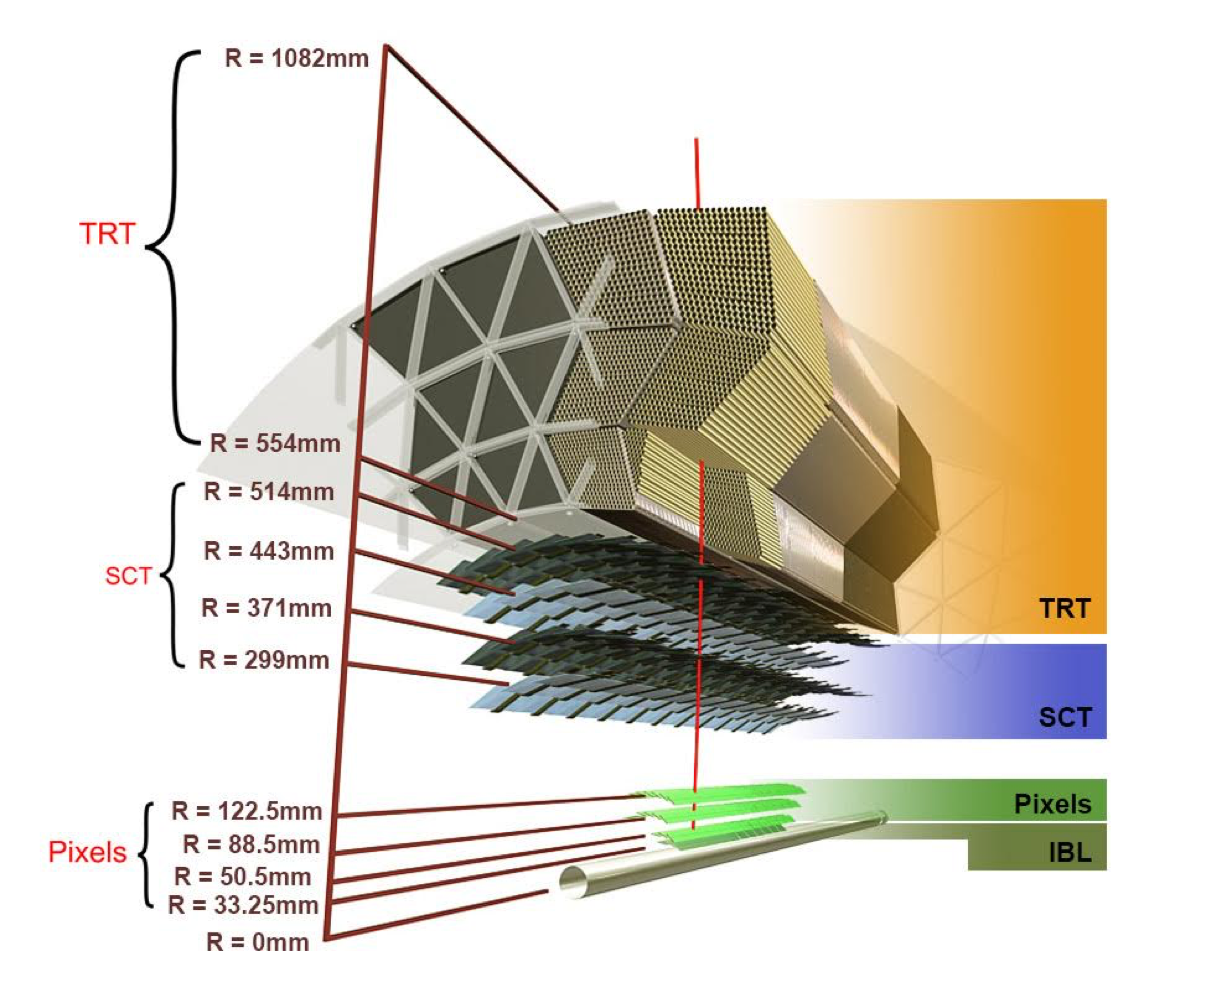
\includegraphics[width=0.8\textwidth]{LHC_ATLAS/IDCrossSection}
\caption{Cross section of the inner detector.}
\end{figure}

The ID is is contained within a cylindrical region of radius \SI{1.05}{\m} and lenght \SI{6.2}{\m} about. It is submerged in a \SI{2}{\tesla} solenoidal magnetic field and it consists of three independent and complementary parts which are the pixel detector, SemiConductor Tracker (SCT) and the transition radiation tracker (TRT).

The pixel detector, covering the \AetaRange{2.5} range, is the closest detector from the beam reaching about \SI{33.25}{\mm} in distance with the Insertable B-layer (IBL) added during LS1. The principal task of the ID is to reconstruct primary and secondary verteces. In the barrel region, it is arranged on three concentric cylinders around the beam axis while in the end-cap regions it is located on disks perpendicular to the beam axis. A Pixel sensor is a \si{16.4} $\times$ \SI{60.8}{\mm} wafer of silicon with \num{46080} pixels having a minimum size in $R$-$\phi \times z$ of  \si{50} $\times$ \SI{400}{\um\squared} each. Thanks to its triple layer, the detector provides three measurement points to reconstruct the track with a resolution of \SI{10}{\um} in the direction orthogonal to its disposition and \SI{115}{\um} in the longitudinal one. The pixel detector has approximately \num{92} million readout channels achieving an accuracy of \SI{10}{\um} in the $R$-$\phi$ plane and \SI{150}{\um} in $z$ direction for barrel and in $R$ direction for the end-cap region.

SCT is devoted to reconstruct particles momenta. It spans a $R$ distance between \SI{299}{\mm} and \SI{514}{\mm} and it consists of modules of silicon strips arranged in four concentric barrels and two end-caps of nine disks each. In the barrel it uses small angle stereo strips to measure a particle's coordinates, with a particular set parallel to the beam axis for measuring $R$ and $\phi$, while in the end-cap it uses a set of strips running radially and a set of stereo strips at an angle of \SI{40}{mrad}. Here eight strip layers corresponding to four space points are crossed by each track. The total number of readout channels in the SCT is approximately 6.3 million, each of them providing a precision of \SI{17}{\um} in the $R$-$\phi$ plane and \SI{180}{\um} in $z$ direction for barrel and in $R$ direction for the end-cap region.

The outer part of the ID is TRT which is another cave cilinder of radii \SI{554}{\mm} and \SI{1082}{\mm}. The detecting elements are drift tubes (straws) with a diameter of \SI{4}{mm} and \SI{144}{cm} long in the barrel region, where they are parallel to the beam axis being cut in a half at $\eta =0$, and \SI{37}{\cm} long in the end-cap region where they are distributed radially. It provides information only on $R$-$\phi$ coordinates with a resolution of  only \SI{200}{\um} per straw, much less than the other two detectors. On the other hand it provides a very large number of hits per track, which is about \num{36}. Each straw is held at \SI{-1500}{\V} driving the negative ions, occuring after a charged particle has crossed the gas they're filled with, to a fine wire down the centre of each straw, producing a current in the wire. The ones with signals create a pattern of straws have being hit that allow the determination of the particles path. The TRT has about \num{298000} straws in total.

The combination of precision trackers in the innermost shell with the TRT at a larger radius gives very robust pattern recognition and high precision measurements. For instance the TRT's straws hit at great radius contributes significantly to determine a particle's momentum by compensating their small precision with longer measured track and larger number of hits.

The inner detector system provides tracking measurements in a range matched by the precision measurements of the electromagnetic calorimeter which will be described in the next section.

\subsection{Calorimetry}
\label{sec:calo}
Calorimeters are the detectors dedicated to energy measurements for every particle, except for muons, including the missing transverse energy (\met) whose precise measurement is possible thanks to the wide pseudorapidity range, up tp $\eta=4.9$, while the $\phi$ coverage is full. Nevertheless there is a blind zone in \etaRange{1.37}{1.52} called \emph{crack region} where the barrel/end-cap transition happens.

In ATLAS the calorimetry system, represented in \Fig{\ref{fig:Calos}} is composed by two subsystems: the electromagnetic (EM) calorimeter, devoted to recognize photons and electrons thanks to its finer granularity, and the hadronic calorimeter which accounts for hadrons such jets. Both of them are sample calorimeters, which means they are made as a series of active material and and absorber material.

An important feature in building them is the calorimeter depth. They must provide good containment for electromagnetic and hadronic showers limiting the number of electrons, photons and hadrons break into the muon spectrometer. The total thickness of the EM calorimeter is greater than 22 radiation lengths ($X_0$), which is defined as the mean distance over which a high energy electron loses $1/e$ of its energy by bremsstrahlung, in the barrel and greater than 24 $X_0$ in the end-caps.

\begin{figure}[tp]
\centering
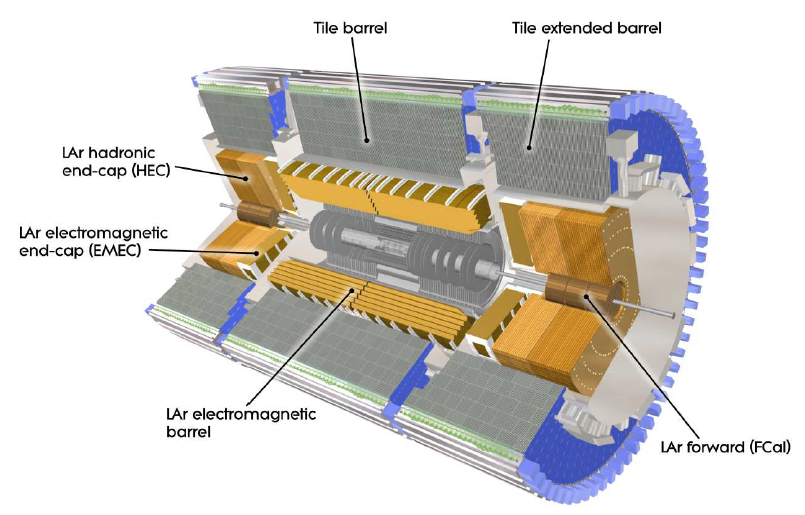
\includegraphics[width=0.8\textwidth]{LHC_ATLAS/Calorimetry}
\caption{Cut-away view of ATLAS calorimetry system. It develops around the inner detector in gray and it is composed by the electromagnetic and hadronic calorimers.}
\label{fig:Calos}
\end{figure}

\subsubsection{Electromagnetic calorimeter}
\begin{figure}[tp]
\centering
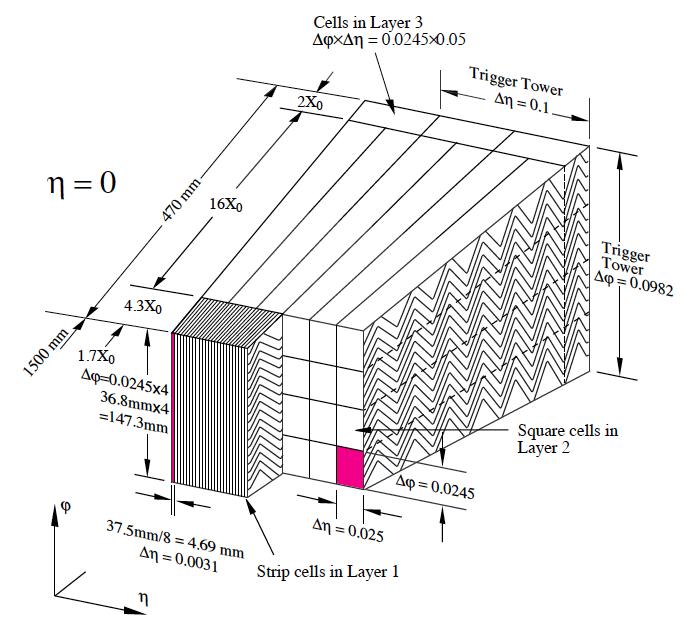
\includegraphics[width=0.55\textwidth]{LHC_ATLAS/EMcalo}
\caption{Schematic view of a fraction of the EM calorimeter showing its accordion geometry and pointing out the segmentation in ``strips'', ``middle'' and ``back'', along with their granularity, in the  barrel region.}
\label{fig:EMlayers}
\end{figure}

The EM calorimeter is designed to detect, measure and track electrons and photons and it is part of the LAr calorimetry. Indeed it adopts entirely this tecnology being made up of a liquid argon ionization chamber using lead as absorber. It is composed by two half-barrels, separated at $\eta=0$ by a \SI{4}{\mm} gap, covering \AetaRange{1.475} and two end-cap regions (EMEC), composed by a outer and an inner weel, extending the range in pseudorapidity to \etaRange{1.375}{3.2} each housed in its own cryostat. 

It is built following an accordion geometry which naturally covers a full $\phi$ simmetry without any cracks. In the barrel the accordion waves are parallel to the beam axis, running in $\phi$, and their folding angle varies with $R$ keeping the LAr gaps pretty constant. In the endcaps, the waves run axially and the folding angle varies with radius.

In the longitudinal direction and for \AetaRange{2.5} where precise measurements take place, the EM barrel calorimeter is segmented into three sections and in the end-cap zone, i.e. the inner wheel, in two sections. In barrel the three sections are called ``strips'', ``middle'' and ``back'' as pictured in \Fig{\ref{fig:EMlayers}}. In the strips the highest granularity is found and it reaches \mbox{$0.008 \times 0.1 \left(\Delta \eta \times \Delta \phi \right)$}, needed to distinguish between a decayed \pizero from an actual photon. The middle calorimeter collects the greater fraction of energy of electromagnetic showers and the back detects its tail and prevents the shower to reach the outer hadronic calorimeter.
  
Going through the ID, energy loss for photons and electrons might happen and it must be taken into account. A presampler, which is a very thin liquid-argon layer ($\sim \SI{11}{\mm}$), is added before the calorimeter to recover any kind of loss.

\subsubsection{Hadronic calorimeter}
The hadronic calorimeter is characterized by two different technology: the tile calorimeter in the barrel region, and the LAr hadronic forward (FCal) and end-cap (HEC) calorimeter. 

The tile calorimeter, placed just outside the EM calorimeter, is a sample calorimeter which uses steel as absorber and a scintillator as an active medium giving a better response time than the LAr technology. It can be divided in the proper barrel region and two extended barrels, both extending from an inner radius of \SI{2.28}{\m} to an outer one of \SI{4.25}{\m} and segmented in depth in three layers. The barrel covers the region \AetaRange{1.0} and the two extended barrels extend the covering by measuring \etaRange{0.8}{1.7}. While speaking of hadrons interaction lenghts ($\lambda$), i.e. the mean distance before hadrons interact with nuclear matter, must be used instead of radiation lenght. The interaction lenght can be computed as $\lambda \simeq \frac{A^{1/3}}{\rho}$ where $A$ is the mass number for a specific atom and $\rho$ is the nuclear density. The total detector thickness in the tile-instrumented region is \SI{9.7}{\lambda} at $\eta = 0$ and \SI{10}{\lambda} in the extended barrel.

The HEC and FCal parts use the same technology as in the EM calorimeter so that their active medium is liquid Argon but their absorber can be tungsten and copper. HEC is located directly behind the EM end-cap calorimeter, sharing the same cryostat, and it consists of two independent wheels per end-cap. Each weel is divided into two segments in depth, for a total of four layers per end-cap. The FCal completes the $\eta$ coverage being located in \etaRange{3.5}{4.9}. It consists of three modules in each end-cap: the first, made of copper, is suited for electromagnetic measurements, while the other two, made of tungsten, measure the energy of hadronic interactions.

\subsection{Muon spectrometer}
\label{sec:muons}
The muon spectrometer is the outermost detector in ATLAS. Its functioning is based on the magnetic deflection of muon tracks in the large superconducting air-core toroid magnets build in such a way the magnetic field is almost orthogonal to muons path. For \AetaRange{1.4} bending is achieved thanks to the barrel toroids, for \AetaRange{1.6}{2.7} muons are bent by two smaller end-cap toroids and int the intermediate, or transition, region for \etaRange{1.4}{1.6} the deflection occurs for a combination of the two fields. Bending power is computed by the field integral $\int B_{\bot}\,dl$ where $B_{\bot}$ is the field perpendicular to the muons trajectory and the integral is evaluated along the infinitesimal path covered by muons inside the spectrometer. The barrel toroid provides \SI{1.5}{\tesla \metre} to \SI{5.5}{\tesla \metre} and the end-cap toroid gives from \SI{1}{\tesla \metre} to \SI{7.5}{\tesla \metre}, while in the transition region the bending power is much lower. The magnetic field is continuously monitored by almost 1800 Hall sensors distributed throughout the spectrometer, this is crucial in order to calculate the bending power along the muon trajectory to a few parts in a thousand.

In the barrel region, tracks are measured in chambers arranged in three cylindrical layers around the beam axis while in transition and end-cap region three-layered chambers are located in planes orthogonal to the $z$-axis. Monitored Drift Tube (MDT) chambers pursue high-precision tracking along almost the whole $\eta$ range. They are made of cylindrical aluminum drift tube being filled with gas which gets ionized when a muon passes by. Charges are collected by a wire held at high potential. Cathode-strip chambers (CSC) covers \etaRange{2}{2.7}. They are multiwire proportional chambers with cathodes segmented into strips with an higher rate capability and greater granularity.

The muon spectrometer has its own trigger system which extends over \AetaRange{2.4} and uses Resistive Plate Chambers (RPC) and Thin-gap Chambers (TGC) in barrel and end-cap regions respectively. What the trigger achieves is bunch crossing identification (BCID), to give a precise \pt threshold and to measure muons tracks in direction orthogonal to which the chambers have measured.

\begin{figure}[pt]
\centering
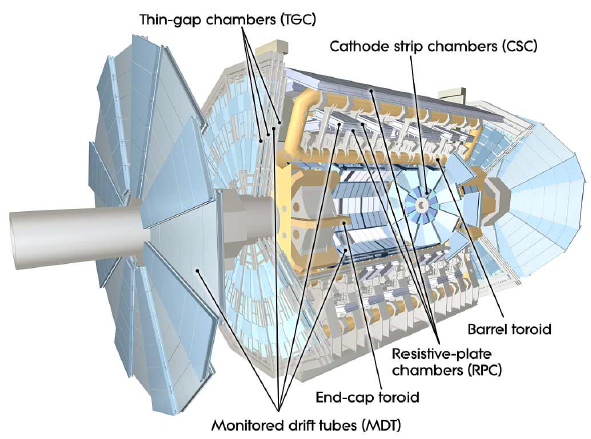
\includegraphics[width=0.75\textwidth]{LHC_ATLAS/Muons}
\caption{Cut-away view of the ATLAS muon system.}
\label{fig:muons}
\end{figure}

\begin{figure}[pt]
\centering
\small
\fontfamily{pag}\selectfont
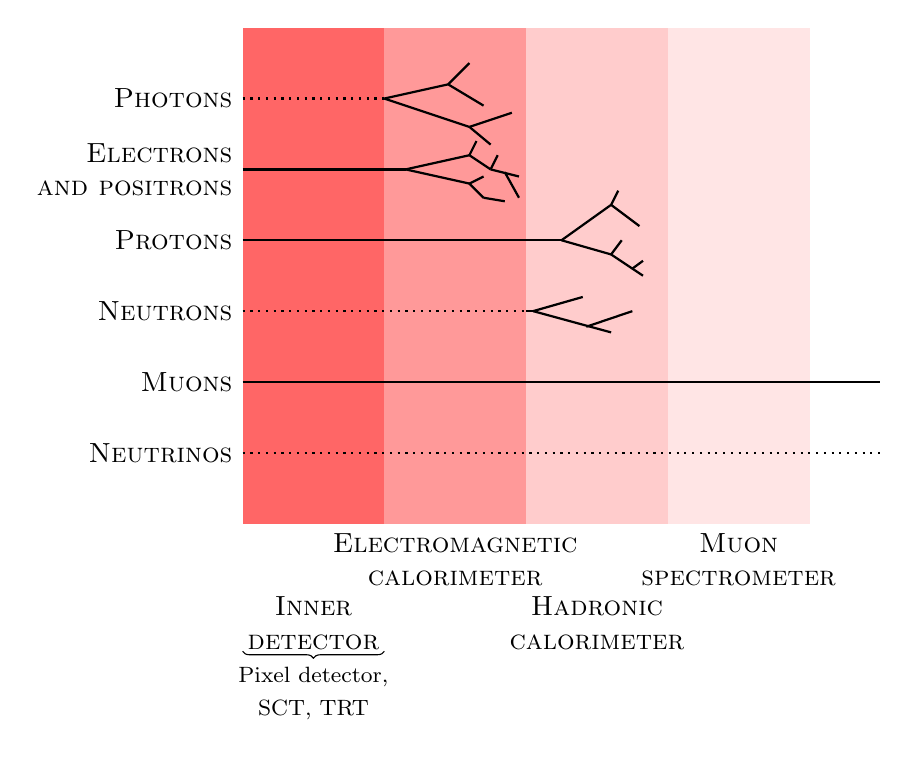
\begin{tikzpicture}[scale=0.9]
	\draw[draw=none,fill=red!60!white] (0,0) rectangle +(2,7);
	\draw[draw=none,fill=red!40!white] (2,0) rectangle +(2,7);
	\draw[draw=none,fill=red!20!white] (4,0) rectangle +(2,7);
	\draw[draw=none,fill=red!10!white] (6,0) rectangle +(2,7);
	
	\draw[thick,dotted] node[left] at (0,6) {\scshape Photons};
		\draw[dotted,thick] (0,6)--(2,6);
		\draw[thick] (2,6)--(2.9,6.2);
			\draw[thick] (2.9,6.2)--(3.2,6.5);
			\draw[thick] (2.9,6.2)--(3.4,5.9);
		\draw[thick] (2,6)--(3.2,5.6);
			\draw[thick] (3.2,5.6)--(3.5,5.35);
			\draw[thick] (3.2,5.6)--(3.8,5.8);
	\draw[thick,dotted] node[left,align=right] at (0,5) {\textsc {Electrons}\\ \textsc{and positrons}} ;
		\draw[thick] (0,5)--(2.3,5);
			\draw[thick] (2.3,5)--(3.2,5.2);
				\draw[thick] (3.2,5.2)--(3.3,5.4);
				\draw[thick] (3.2,5.2)--(3.5,5);
					\draw[thick](3.5,5)--(3.6,5.2);
					\draw[thick](3.5,5)--(3.9,4.9);
						\draw[thick](3.7,4.96)--(3.9,4.6);
			\draw[thick] (2.3,5)--(3.2,4.8);
				\draw[thick] (3.2,4.8) --(3.4,4.9);
				\draw[thick] (3.2,4.8) --(3.4,4.6);
					\draw[thick] (3.4,4.6) -- (3.7,4.55);
	
	\draw[thick,dotted] node[left,align=right] at (0,4) {\textsc{Protons}};
		\draw[thick] (0,4)--(4.5,4);
			\draw[thick] (4.5,4) -- (5.2,4.5);
				\draw[thick] (5.2,4.5)--(5.3,4.7);
				\draw[thick] (5.2,4.5)--(5.6,4.2);
			\draw[thick] (4.5,4) -- (5.2,3.8);
				\draw[thick] (5.2,3.8) -- (5.35,4);
				\draw[thick] (5.2,3.8) -- (5.5,3.6);
					\draw[thick] (5.5,3.6) -- (5.65,3.71);
					\draw[thick] (5.5,3.6) -- (5.65,3.5);
	\draw[thick,dashed] node[left] at (0,3) {\scshape Neutrons};
		\draw[thick,dotted] (0,3)--(4,3);
		\draw[thick] (4,3)--(4.1,3);
			\draw[thick] (4.1,3)--(4.8,3.2);
			\draw[thick] (4.1,3)--(5.2,2.7);
				\draw[thick] (4.85,2.78)--(5.5,3);
	
	\draw[thick] node[left] at (0,2) {\scshape Muons} (0,2) -- (9,2);	
	\draw[thick,dotted] node[left] at (0,1) {\scshape Neutrinos} (0,1) -- (9,1);
	
	\node[align=center] at (1,-1.4) {\scshape Inner\\ \scshape detector};
	\node[align=center] at (3,-.5) {\scshape Electromagnetic\\ \scshape calorimeter};
	\node[align=center] at (5,-1.4) {\scshape Hadronic\\ \scshape calorimeter};
	\node[align=center] at (7,-.5) {\scshape Muon\\ \scshape spectrometer};
	\draw [decorate,decoration={brace}] (2,-1.8)--(0,-1.8);
	\node[align=center] at (1,-2.4) {\footnotesize Pixel detector,\\ \footnotesize SCT, TRT};
\end{tikzpicture}
\caption{Particle behavior inside the various parts of the ATLAS detector, dotted lines are invisible to the various detectors.}
\label{fig:behaviour}
\end{figure}

\begin{table}[tp]
	\centering
	\begin{tabular}{lc}
	\toprule
	Detector & Pseudorapidity range\\
	\midrule
	Inner detector& \AetaRange{2.5}\\
	EM calorimeter barrel& \AetaRange{1.475}\\
	EM calorimeter end-cap& \etaRange{1.375}{3.2}\\
	Hadronic tile calorimeter barrel& \AetaRange{1.0}\\
	Hadronic tile calorimeter extended barrel& \etaRange{0.8}{1.7}\\
	Hadronic end-cap calorimeter (HEC)& \etaRange{1.5}{3.2}\\
	Hadronic Forward calorimeter (FCAL)& \etaRange{3.1}{4.9}\\
	Muon spectrometer& \AetaRange{2.7}\\
	\bottomrule
	\end{tabular}
	\caption{Table listing the pseudorapidity range for every part of the ATLAS detector}

\end{table}
\subsection{Forward calorimeters}
Three smaller detector systems cover the ATLAS forward region. LUCID (LUminosity measurement using Cerenkov Integrating Detector) at \SI{\pm 17}{\m}, along the beam, and ALFA (Absolute Luminosity For ATLAS) located at \SI{\pm 240}{\m} are used to measure the istantaneous luminosity delivered to ATLAS. The former by detecting inelastic \pp scattering while the latter by using scintillating fiber trackers inside Roman pots capable to reach \SI{1}{mm} from the beam. The third system is the Zero-Degree Calorimeter (ZDC), located at \SI{\pm 140}{\m}, which is used in determining the centrality of heavy-ion collisions.

\subsection{Trigger system}
The rate of events expected rate at the LHC designed luminosity is \SI{1}{\GHz}, as mentioned in the previous Section, on the other hand the maximum event rate that ATLAS can record is \SI{\sim 200}{\MHz}. It is evident that an appropriate trigger system must be used so that only events that could have potential physical interest would be recorded. There are three distinct levels of trigger: L1, L2 and the event filter. Each trigger level refines the decisions made at the previous level using greater amount of data at each step, and, where necessary, applies additional selection criteria.

L1 looks for high-\pt particles such as electrons, photons, $\tau$-leptons decaying into hadrons as well as large \met and defines one or more Region-of-Interest (RoI) which is a $\Delta \eta \times \Delta \phi$ region in which interesting events can be found. It uses information coming from a subset of detectors which are processed by the central trigger processor. The operating time is about \SI{2.5}{\um} which reduces the event rate down to \SI{100}{\kHz}.

L2 elaborates all the subdetector information in a particular RoI. It uses a more complicate algorithm than L1 and it can reduce the event rate to \SI{4}{\kHz}. It provides a first full reconstruction of the events made by the Event Builder which uses its informations.

The final stage of the selection is made by the Event Filter (EF) which reduces the rate to a reasonable \SI{200}{\Hz}. It selects events using the full granularity avaliable for each subdetector, and store them as raw data (RDO) for offline analysis. Every event is computed in about \SI{4}{\s}.




